\section{Sprint 1.1 : Initialisation, authentification et gestion des permissions}
Ce premier sprint a couvert quatre axes majeurs :
\begin{itemize}[label=$-$]
    \item \textbf{Initialisation du projet} : création du dépôt Git, configuration des outils de travail, structuration du projet, ainsi que compréhension et analyse du code de l’ancienne application.
    \item \textbf{Développement de la page d’accueil} destinée aux visiteurs.
    \item \textbf{Authentification et gestion des profils} :
    \item \textbf{Gestion des utilisateurs} : développement des fonctionnalités permettant d’afficher la liste des utilisateurs, de consulter leurs informations et de gérer leurs rôles ou autorisations.
\end{itemize}
\subsection{Backlog du sprint 1.1}  
Cette section présente le backlog du sprint 1.1, comme illustré dans le tableau \ref{tab:backlogS11}.
\begin{landscape}
    \renewcommand{\arraystretch}{1.37}
    \begin{spacing}{0.94}
        \begin{longtable}{|p{0.7cm}|p{2.4cm}|p{6cm}|p{1cm}|p{7.2cm}|p{0.2cm}|p{0.2cm}|p{2cm}|}
            \caption{Backlog du sprint 1.1} \label{tab:backlogS11} \\\hline
            \rowcolor{gray!20}
            \textbf{\small ID US} & 
            \multicolumn{1}{c|}{\textbf{\small User Story}} & 
            \multicolumn{1}{c|}{\textbf{\small Description}} & 
            \textbf{\small ID tâche}& 
            \multicolumn{1}{c|}{\textbf{\small Tâches}} & 
            \multicolumn{1}{c|}{\textbf{\small Priorité}} & 
            \multicolumn{1}{c|}{\textbf{\small Risques}} & 
            \textbf{\small Estimation (Jours)}\\\hline
            % ----------- INITIALISATION ------------------
            \hline  
            \rowcolor{blue!20}
			\multicolumn{8}{|c|}{\textbf{EPIC 1: Initialisation du projet}} \\\hline
            1.1 & Installation de l’environnement de travail 
                  & En tant que développeur, je dois installer les outils nécessaires pour travailler. & 1.1.A \newline\vspace{0.5cm} 1.1.B
            & - Installer Python, VSCode, Docker, Git, npm, Angular...\newline
            - Configurer l'environnement. & Élevée & Basse & 1 \\\hline
            1.2 & Formation Scrum. 
                  & En tant que développeur, je dois être formé à la méthodologie Scrum afin d’organiser le travail. 
              & 1.2.A & 
                - Participer à une session de formation SFC de SCRUMstudy. et passer un test pour obtenir la certification.\footnote{Voir annexe B: Figures \ref{fig:ProgressionCours} et \ref{fig:CertifSRC}}
        & Basse & Basse & 2 \\
            \hline
        1.3 & Formation aux tests de pénétration. 
            & En tant que développeur, je dois être formé aux principes du pentesting pour comprendre les besoins de sécurité. 
            & 1.3.A \newline1.3.B 
            & 
            - Étudier les techniques de pentesting. \newline
            - Trouver les principaux outils de base de pentesting Web et les vulnérabilités les plus courantes.
            & Élevée & Basse & 3  \\
            \hline
            1.4 & Formation Selenium. 
                  & En tant que développeur, je dois être formé à l’automatisation avec Selenium pour automatiser les tests fonctionnels. 
                & 1.4.A \newline1.4.B \newline 1.4.C 
                & 
                - Suivre une formation Selenium. \newline
                - Installer et configurer Selenium. \newline
                - Comprendre les bases de la manipulation des éléments Web. 
                & Élevée & Basse & 3 \\\hline
            1.5 & Analyse de la solution existante. 
                  & En tant que développeur, je dois analyser la solution existante pour identifier les fonctionnalités et les limites.
                  & 1.5.A \newline\vspace{0.5cm} 1.5.B 
                & 
                - Analyser la solution existante et identifier ses limites.
                \newline
                - Formaliser les besoins utilisateurs en spécifications fonctionnelles.& Élevée & Moyenne & 3\\
            \hline
            1.6 & Formation RabbitMQ. 
                & En tant que développeur, je dois suivre une formation sur RabbitMQ afin de comprendre le fonctionnement de la communication asynchrone entre services. 
                & 1.6.A \newline\vspace{0.9cm} 1.6.B 
                & 
                - Étudier les concepts de base de RabbitMQ (file d’attente, échange, routage). \newline
                - Installer RabbitMQ en local et tester la communication entre deux services via des files de messages.
                & Élevée & Moyenne & 3 \\
            \hline
            % ----------- CONSULTATION PAGE D’ACCUEIL ------------------
            \hline  
            \rowcolor{blue!20}
            \multicolumn{8}{|c|}{\textbf{EPIC 2: Consultation de la page d’accueil}} \\\hline
            2.1 & Accéder à la page d’accueil 
            & En tant que visiteur, je souhaite accéder à la page d’accueil sans avoir besoin de créer un compte. 
            & 2.1.A 
            &
            - Configurer l’accès libre à la page d’accueil depuis l’URL principale. 
            & Moyenne & Basse & 1/2 \\ \hline
            
            2.2 & Parcourir les sections de la page d’accueil 
            & En tant que visiteur, je souhaite consulter les sections publiques (FAQ, guide utilisateur, services, équipe, tarification, etc.) pour m’informer. 
            & 2.2.A \newline\vspace{0.5cm}2.2.B 
            &
            - Développer les sections publiques avec leur contenu respectif. \newline
            - Intégrer les textes descriptifs, images et icônes explicatives. 
            & Moyenne & Moyenne & 4 \\ \hline
            
            2.3 & Soumettre une demande de contact
            & En tant que visiteur, je souhaite envoyer un message via un formulaire pour poser une question ou obtenir de l’aide. 
            & 2.3.A 
            &
            - Implémenter un formulaire de contact avec champs (nom, e-mail, message) et envoi vers l’administrateur. 
            & Moyenne & Moyenne & 1/2 \\ \hline
            
            % ----------- AUTHENTIFICATION ------------------
            \hline  
            \rowcolor{blue!20}
			\multicolumn{8}{|c|}{\textbf{EPIC 3: Authentification et gestion du profil }} \\\hline
            3.1 & S'inscrire 
            & En tant que visiteur, je dois créer un compte afin d'accéder à l'application. 
            & 3.1.A
            &
            - Implémenter un formulaire d'inscription avec validation et gestion des tokens pour sécuriser les accès. 
            & Moyenne & Moyenne & 1 \\ \hline
            3.2 & Vérifier l’adresse e-mail après l’inscription. 
                & En tant que visiteur, je dois recevoir un lien de vérification afin de valider mon compte et sécuriser l'accès. 
                & 3.2.A \newline\vspace{0.5cm} 3.2.B 
                &
                - Générer un lien de vérification unique après l'inscription. \newline
                - Implémenter un service pour envoyer l'email de vérification. 
                & Moyenne & Moyenne & 1/2 \\ \hline
            3.3 & S’authentifier
                & En tant qu’un utilisateur, je veux pouvoir me connecter pour gérer mon accès. 
                & 3.3.A&
                - Mettre en place une page de connexion avec un formulaire d’authentification et validation des identifiants.
                & Moyenne & Basse & 1/2 \\ \hline
            3.4 & Réinitialiser le mot de passe en cas d’oubli. 
                & En tant qu’un utilisateur, je veux réinitialiser mon mot de passe si je l'oublie, pour retrouver l'accès. 
                & 3.4.A \newline\vspace{0.5cm} 3.4.B 
                &
                - Créer une page de réinitialisation de mot de passe. \newline
                - Implémenter la validation par email pour réinitialiser le mot de passe. 
                & Moyenne & Moyenne & 1 \\ \hline
            3.5 & Gérer le profil utilisateur. 
                & En tant qu’un utilisateur, je veux modifier mes informations personnelles pour garder mes données à jour. 
                & 3.5.A \newline\vspace{0.5cm} 3.5.B 
                &
                - Créer une page pour modifier les informations personnelles. \newline
                - Implémenter la mise à jour des utilisateur dans la base de données. 
                & Moyenne & Moyenne & 1/2 \\\hline
              3.6 & Se déconnecter 
                & En tant qu’un utilisateur, je veux me déconnecter de l’application.
                & 3.6.A
                &
                - Implémenter un bouton de déconnexion sur l’interface frontend avec suppression du jeton de session. 
                & Moyenne & Basse & 1/2 \\  \hline
            \hline     
            % ---- GESTION DES UTILISATEURS -----------
            \hline  
            \rowcolor{blue!20}
			\multicolumn{8}{|c|}{\textbf{EPIC 11: Gestion des utilisateurs}} \\\hline
            11.1 & Rechercher un utilisateur 
            & En tant qu’administrateur, je souhaite rechercher un utilisateur avec différents filtres pour retrouver rapidement un profil. 
            & 11.1.A 
            & - Implémenter un champ de recherche avec filtres (nom, email, rôle…). 
            & Élevée & Moyenne & 1/2 \\\hline
            
            11.2 & Exporter la liste des utilisateurs 
            & En tant qu’administrateur, je souhaite exporter la liste des utilisateurs afin de la conserver.
            & 11.2.A 
            & - Générer un export (PDF/CSV/HTML /JSON) de la liste des utilisateurs. 
            & Moyenne & Basse & 1/2 \\\hline
            
            11.3 & Consulter la liste des utilisateurs 
            & En tant qu’administrateur, je souhaite voir la liste des utilisateurs pour une vue globale. 
            & 11.3.A 
            & - Afficher un tableau paginé listant les comptes avec leurs informations principales. 
            & Moyenne & Basse & 1/4 \\\hline
            11.4 & Supprimer un utilisateur 
            & En tant qu’administrateur, je souhaite pouvoir supprimer un utilisateur du système. 
            & 11.4.A 
            & - Ajouter un bouton de suppression avec confirmation de sécurité. 
            & Élevée & Moyenne & 1/4 \\\hline
            
            11.5 & Gérer les permissions des utilisateurs
            & En tant qu’administrateur, je souhaite attribuer, modifier ou révoquer les permissions d’un utilisateur afin de contrôler ses droits d’accès.
            & 11.5.A 
            \newline\vspace{1.9cm} 11.5.B
             \newline\vspace{0.5cm} 11.5.C
            & - Créer une interface permettant d’attribuer, modifier, révoquer et visualiser les permissions d’accès aux différents types de scans (fonctionnel, SEO, sécurité) pour chaque utilisateur.\newline
            - Implémenter des vérifications côté backend sur les routes sensibles.\newline
            - Restreindre l’accès selon les permissions via des guards côté frontend.
            & Élevée & Moyenne & 1/2 \\\hline

            \rowcolor{gray!20}
			\multicolumn{7}{|c|}{TOTAL} &  26UE \\
            \hline 
        \end{longtable}
    \end{spacing}
    \vspace{-0.1cm}
\end{landscape}

\subsection{Analyse du sprint 1.1}
Nous passons à la phase d’analyse de ce sprint afin de présenter le diagramme de cas d’utilisation de ce sprint ainsi que les descriptions textuelles de quelques cas d’utilisation. 
\subsubsection{Diagramme de cas d’utilisation du sprint 1.1}
La figure \ref{fig:caseS1} présente le diagramme de cas d’utilisation raffiné du sprint 1.1, mettant en évidence les cas d’usage correspondant aux fonctionnalités attendues à la fin de ce sprint.
\begin{figure}[H]
    \centering
    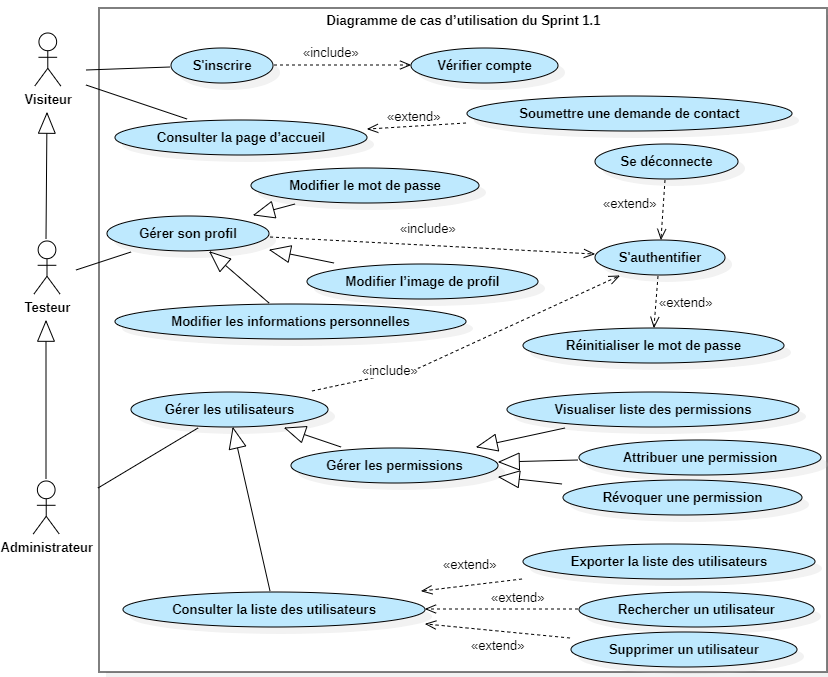
\includegraphics[width=0.92\linewidth]{chapitres/ch3Sp1/section/sprint1/img/LastUseCaseSprint1.1.png}
    \caption{Diagramme de cas d’utilisation du sprint 1.1}
    \label{fig:caseS1}
\end{figure}
\vspace{-0.5cm}
\subsubsection{Raffinement des cas d’utilisation}
Cette étape a permis de mieux comprendre les interactions, de repérer les dépendances et de découper les fonctionnalités.
\begin{enumerate}[label=\alph*), left=-0.1cm]
    \item \textbf{Raffinement du cas d’utilisation «S'inscrire»:}\\
        L'inscription inclut la saisie et validation des informations, la confirmation par e-mail avec un code OTP et la gestion des erreurs pour garantir une expérience utilisateur optimale.
        \begin{itemize}[label=\ding{111}, left=-0.1cm]
            \item \textbf{Description textuelle du cas d’utilisation "S'inscrire":} \\
                  Le tableau ~\ref{tab:descInsc}  présente la description textuelle du cas d’utilisation "S'inscrire".
                  \begin{spacing}{1.1}
                        \begin{longtable}{|p{0.12\linewidth}|p{0.88\linewidth}|}
                            \caption{Description textuelle du cas d’utilisation : S'inscrire}
                            \label{tab:descInsc}\\
                            \hline
                            \textbf{Titre} & S'inscrire \\
                            \hline
                            \textbf{Acteur} & Visiteur \\
                            \hline
                            \textbf{Résumé} & Ce cas d'utilisation décrit le processus d'inscription permettant au visiteur de créer un compte personnel. \\
                            \hline
                            \textbf{Pré-conditions} & 
                                Le visiteur doit disposer d’un accès à Internet via un dispositif connecté (ordinateur, tablette, smartphone). \\
                            \hline
                            \textbf{Post-conditions} & 
                                Un nouveau compte utilisateur est créé, et un email de confirmation contenant un code OTP est envoyé afin de vérifier l’adresse email saisie. \\
                            \hline
                            \textbf{Scénario nominal} & 
                            \begin{minipage}{\linewidth}
                                \vspace{0.1cm}
                                \begin{enumerate}[label=\arabic*., left=-0.05cm]
                                    \item Le visiteur accède à la page d'inscription et clique sur le bouton "Inscrire".
                                    \item Le système affiche un formulaire de saisie des informations d'inscription.
                                    \item Le visiteur remplit le formulaire avec ses informations, puis le soumet.
                                    \item Le système valide les informations fournies.
                                    \item Le système enregistre les données du visiteur dans la base de données.
                                    \item Il génère automatiquement des identifiants de connexion.
                                    \item Le système envoie un e-mail de confirmation contenant un code OTP (One-Time Password) de 6 chiffres.
                                    \item L'utilisateur saisit ce code dans un champ dédié.
                                    \item Une fois le code validé avec succès, l'adresse e-mail est vérifiée et l'inscription est finalisée.
                                \end{enumerate}
                                \vspace{0.05cm}
                            \end{minipage}\\
                            \hline
                            \textbf{Scénario d’erreur} &
                            \begin{minipage}{\linewidth}
                                \vspace{0.1cm}
                                \begin{itemize}[left=0cm]
                                    \item[\textbullet] \textbf{Étape 4 (Informations incomplètes):}
                                    \begin{itemize}[label=\ding{56}]
                                        \item Si des champs obligatoires sont laissés vides, le système affiche un message d’erreur précisant les champs à compléter.
                                        \item L'utilisateur est invité à fournir les informations manquantes.
                                    \end{itemize}
                        
                                    \item[\textbullet] \textbf{Étape 4 (Annulation) :}
                                    \begin{itemize}[label=\ding{56}]
                                        \item L'utilisateur peut annuler l'inscription avant la soumission. Aucun enregistrement n’est effectué.
                                    \end{itemize}
                        
                                    \item[\textbullet] \textbf{Étape 7 (Erreur d'enregistrement):}
                                    \begin{itemize}[label=\ding{56}]
                                        \item En cas d’échec lors de l’enregistrement des données, le système affiche un message d’erreur et invite à réessayer ultérieurement.
                                    \end{itemize}
                        
                                    \item[\textbullet] \textbf{Étape 9  (Expiration du code OTP) :}
                                    \begin{itemize}[label=\ding{56}]
                                        \item Le code OTP possède une durée de validité limitée. En cas de dépassement, un message informe l’utilisateur de l’expiration du code et lui propose d’en générer un nouveau via le lien contenu dans l’e-mail.
                                    \end{itemize}
                        
                                    \item[\textbullet] \textbf{Étape 10 (Code OTP incorrect):}
                                    \begin{itemize}[label=\ding{56}]
                                        \item Si l'utilisateur saisit un code OTP erroné, le système affiche un message d'erreur et l'invite à le ressaisir.
                                        \item Après plusieurs tentatives échouées, le système bloque temporairement la validation par OTP et propose l'envoi d'un nouveau code.
                                    \end{itemize}
                                \end{itemize}
                                \vspace{0.1cm}
                            \end{minipage}\\
                            \hline
                        \end{longtable}
                    \end{spacing}
                  \vspace{-0.2cm}
            \item \textbf{Diagramme  de séquence du cas d’utilisation "S'inscrire":} \\ Les étapes de déroulement du cas d’utilisation "S'inscrire" sont décrites par le diagramme de séquence illustré par la figure ~\ref{fig:seqInscrire}.
            \begin{figure}[H]
                \centering
                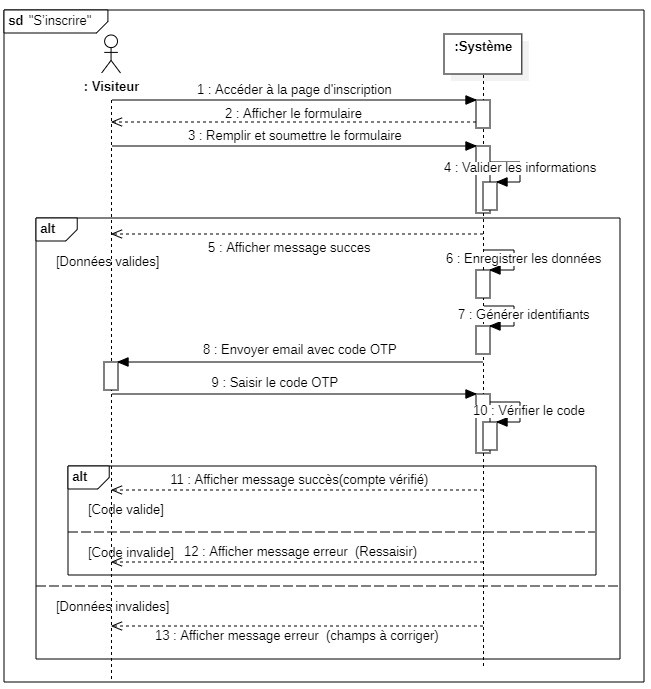
\includegraphics[width=0.9\textwidth]{chapitres/ch3Sp1/section/sprint1/img/seq-creer-compte-sp1.png}
                \caption{Diagramme de séquence du cas d’utilisation de "S'inscrire"}
                \label{fig:seqInscrire}
            \end{figure}
        \end{itemize}
    
  \item \textbf{Raffinement du cas d’utilisation « Gérer les permissions des utilisateurs » :}\\
    Cette section détaille le raffinement du cas d’utilisation « Gérer les permissions des utilisateurs ». Ce cas d’utilisation permet à un administrateur de gérer les droits d’accès des utilisateurs aux différentes permissions (fonctionnel, SEO, sécurité...).
     \begin{itemize}[label=\ding{111}, left=-0.1cm]
            \item \textbf{Description textuelle du cas d’utilisation "Attribuer des permissions" :}\\
            Le tableau \ref{tab:descAttribuerPermissions} décrit textuellement le cas d’utilisation <<Attribuer des permissions>>.
            \begin{spacing}{1.2}
                \begin{longtable}{|p{0.12\linewidth}|p{0.88\linewidth}|}
                \caption{Description textuelle du cas d’utilisation : Attribuer des permissions}
                \label{tab:descAttribuerPermissions} \\
                \hline
                \textbf{Titre} & Attribuer des permissions \\
                \hline
                \textbf{Acteur} & Administrateur \\
                \hline
                \textbf{Résumé} & Ce cas d'utilisation permet à l’administrateur d’attribuer à un utilisateur des permissions d’accès aux tests (fonctionnel, SEO, sécurité). \\
                \hline
                \textbf{Pré-conditions} & L’utilisateur concerné doit exister dans le système. L’administrateur doit être connecté. \\
                \hline
                \textbf{Post-conditions} & Les permissions sélectionnées sont enregistrées et appliquées à l’utilisateur dans la base de données. \\
                \hline
                \textbf{Scénario nominal} &
                \begin{minipage}{\linewidth}
                \vspace{0.1cm}
                \begin{enumerate}[label=\arabic*., left=0.2cm]
                    \item L’administrateur accède à l’interface de gestion des permissions.
                    \item Il sélectionne un utilisateur.
                    \item Il choisit les permissions à autoriser.
                    \item Il valide la configuration.
                    \item Le système enregistre les nouvelles permissions.
                \end{enumerate}
                \vspace{0.1cm}
                \end{minipage} \\
                \hline
                \textbf{Scénario d’erreur} &
                \begin{minipage}{\linewidth}
                    \vspace{0.1cm}
                    \begin{itemize}[left=0cm]
                        \item[\textbullet] \textbf{Erreur d’enregistrement :} En cas d’échec d’écriture en base de données, le système signale une erreur et annule l’opération.
                    \end{itemize}
                    \vspace{0.1cm}
                \end{minipage} \\
                \hline
                \end{longtable}
            \end{spacing}
            \vspace{-0.2cm}
            \item  \textbf{Diagramme d’activité : Vérification des permissions d’accès:}\\
                Le diagramme d’activité de la figure \ref{fig:permission-activite} illustre le processus de gestion conditionnelle des droits d’accès. Après l’authentification, le système accorde aux administrateurs un accès complet leur permettant d’attribuer des permissions.
            \begin{figure}[H]
        \centering
        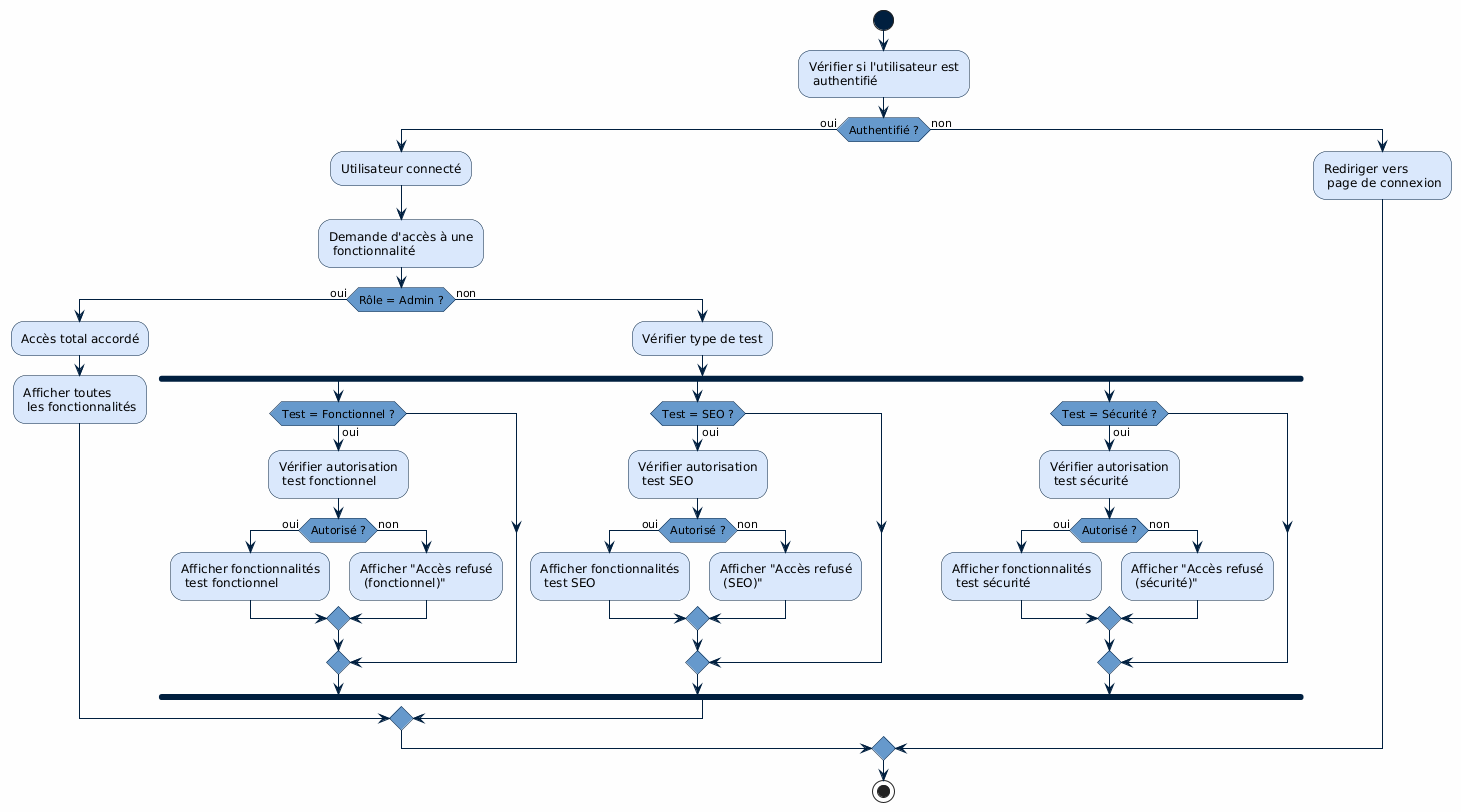
\includegraphics[width=\linewidth]{chapitres/ch3Sp1/section/sprint1/img/permission-activite.png}
        \caption{\centering Diagramme d’activité : Processus de vérification des permissions lors de la demande d’accès à une fonctionnalité}
        \label{fig:permission-activite}
    \end{figure}
    \end{itemize}
    \vspace{-0.5cm}
\end{enumerate}

\subsection{Conception du sprint 1.1}
La conception de ce sprint commence par la présentation du diagramme de classes, représentant la structure du système.
\subsubsection{Diagramme de classe du sprint 1.1}
La figure \ref{fig:classsp1} illustre le diagramme de classes du sprint 1.1, représentant les principales entités métier, leurs attributs, leurs méthodes, ainsi que les relations entre elles.
\begin{figure}[H]
    \centering
    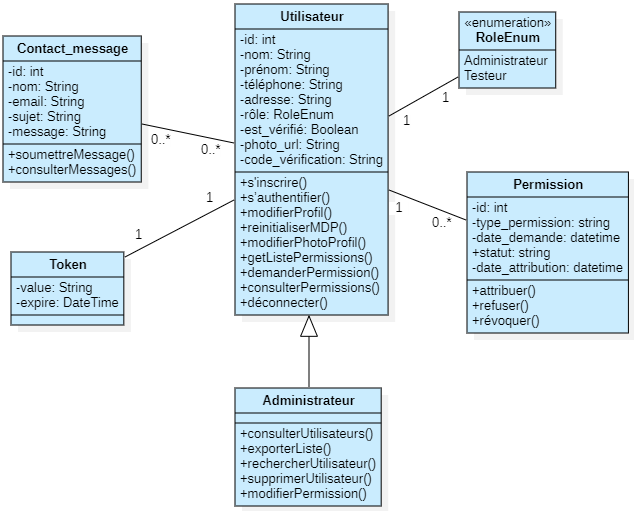
\includegraphics[width=0.9\linewidth]{chapitres/ch3Sp1/section/sprint1/img/classeL1-SP1.1.png}
    \caption{Diagramme de classe du sprint 1.1}
    \label{fig:classsp1}
\end{figure}
\vspace{-0.4cm}
Les principales classes modélisées de sprint 1.1 sont les suivantes:
    \begin{itemize}[label=$*$]
       \item \textbf{Utilisateur :} Représente les comptes utilisateurs de l’application. Elle contient des informations personnelles (nom, prénom, téléphone, adresse, email, mot de passe, et rôle (\texttt{RoleEnum}) ainsi que des méthodes relatives à la gestion du compte et d’administration des utilisateurs.
       \item \textbf{Contact\_message :} Permet aux utilisateurs de soumettre des messages via un formulaire de contact. Elle comprend des attributs et des méthodes pour stocker les détails du message.
       \item \textbf{RoleEnum (énumération) :} Définit les différents rôles possibles dans l’application, notamment \textit{Administrateur} et \textit{Testeur}, utilisés pour la gestion des droits d’accès.
       \item \textbf{Permission :} Représente les permissions associées aux utilisateurs, avec les attributs suivants : type de permission, date de demande, date d’attribution, statut, ainsi que les méthodes : révoquer, attribuer et refuser une demande de permission.
       \item \textbf{Token :} Modélise un jeton d’authentification, avec ses valeurs et sa date d’expiration, utilisé pour la gestion des sessions utilisateurs.
       \item \textbf{Administrateur :} Hérite de la classe Utilisateur et dispose de méthodes spécifiques pour la gestion des utilisateurs, comme consulter la liste des utilisateurs, rechercher, modifier leurs permissions, supprimer des utilisateurs, et exporter la liste.
    \end{itemize}
Les associations entre classes sont également représentées dans le diagramme, notamment:
\begin{itemize}[label=$-$, left=0.05cm]
    \item Un \texttt{Utilisateur} possède un rôle défini par \texttt{RoleEnum} et peut avoir plusieurs \texttt{Permission}.
    \item Un \texttt{Administrateur} : utilisateur disposant de privilèges étendus pour la gestion des autres comptes.
    \item Un \texttt{Utilisateur} peut générer un ou plusieurs \texttt{Token} pour gérer ses sessions.
    \item Un \texttt{Utilisateur} peut envoyer un \texttt{Contact\_message} à plusieurs administrateurs, tandis qu’un \texttt{Administrateur} peut recevoir des messages envoyés par plusieurs utilisateurs.
\end{itemize}
Ce diagramme constitue une base essentielle pour la suite du développement, en assurant une structure cohérente et maintenable du code tout au long des itérations agiles.


\subsection{Réalisation du sprint 1.1}
Dans cette section, nous présentons les principales interfaces développées durant ce premier sprint, en commençant par la page d’accueil, puis celles liées au module d’authentification, et enfin les interfaces de contact et d'administration des utilisateurs.
\begin{itemize}[label=$\bullet$]
    \item  \textbf{Interface de la page d’accueil}: Les figures\footnote{Voir annexe E : Figures \ref{fig:accueil} et \ref{fig:accueil2}} \ref{fig:accueil} et \ref{fig:accueil2} illustrent l’interface de la page d’accueil de l’application. Celle-ci offre un aperçu général du système, avec un design moderne et une navigation intuitive, permettant aux utilisateurs de découvrir rapidement les principales fonctionnalités de la plateforme.
    \item \textbf{Interface d’inscription}:
        La figure~\ref{fig:register} illustre l’interface d’inscription. Elle permet à un nouvel utilisateur de créer un compte en renseignant ses informations personnelles. Des contrôles de saisie assurent la validation des données entrées.  
        \begin{figure}[H]
            \centering
            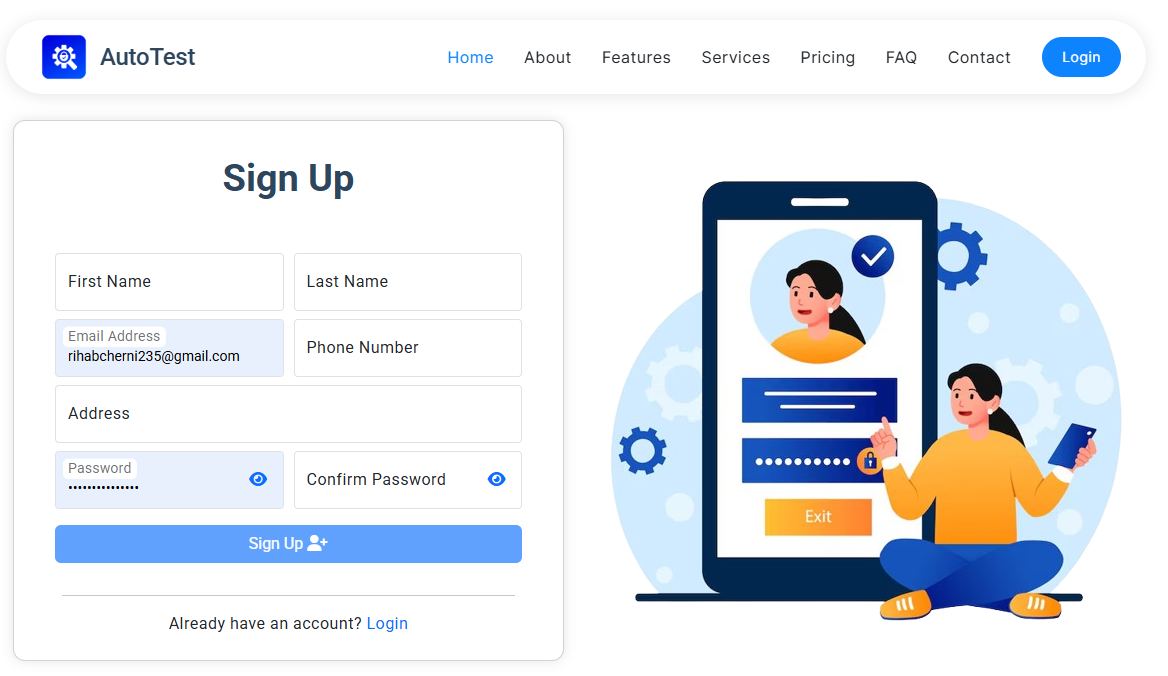
\includegraphics[width=\linewidth]{chapitres/ch3Sp1/section/sprint1/img/interface/register.png}
            \caption{\centering Interface d'inscription}
            \label{fig:register}
        \end{figure}
        \vspace{-0.3cm}
    \item \textbf{Interface de connexion}:
        La figure~\ref{fig:login}\footnote{Voir annexe E: Figures \ref{fig:login}} présente l’interface de connexion. Elle permet à l’utilisateur de s’authentifier via son e-mail et son mot de passe. Des vérifications sont mises en place pour gérer les erreurs (identifiants invalides, champs manquants...).
    \item \textbf{Vérification par e-mail (OTP)}:
        Après l’inscription, l’utilisateur reçoit un e-mail contenant un code de vérification. Les figures \ref{fig:email-verif}\footnote{Voir annexe E: Figures \ref{fig:email-verif}} et \ref{fig:email-verification}\footnote{Voir annexe E: Figures \ref{fig:email-verification}} présentent l’interface de réception et de saisie du code.
    \item \textbf{Mot de passe oublié et réinitialisation}:
        Le système inclut une fonctionnalité de récupération de mot de passe. Les interfaces correspondantes sont illustrées dans les figures~\ref{fig:forgot-password}\footnote{Voir annexe E: Figures \ref{fig:forgot-password}},~\ref{fig:reset-password-email}\footnote{Voir annexe E: Figures \ref{fig:reset-password-email}} et~\ref{fig:reset-password}\footnote{Voir annexe E: Figures \ref{fig:reset-password}}.
        \item \textbf{Profil utilisateur} : La figure~\ref{fig:profile} présente l’interface du profil utilisateur. Chaque utilisateur peut consulter et modifier ses informations personnelles (nom, image de profil, etc.), ainsi que visualiser les permissions qui lui sont attribuées. \\ Un bouton dédié permet également à l’utilisateur de soumettre une demande d’accès à des permissions supplémentaires via une boîte de dialogue affichant la liste des permissions disponibles, que l’utilisateur peut sélectionner avant de valider sa demande.
         \begin{figure}[H]
                \centering
                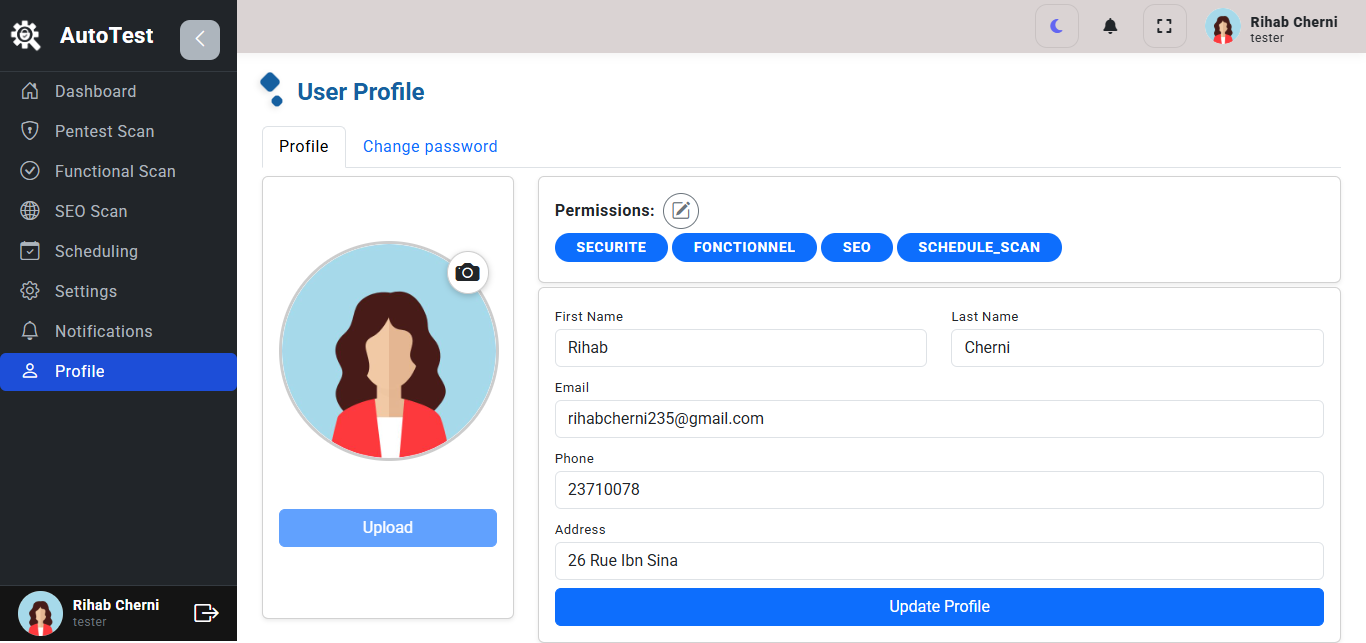
\includegraphics[width=\linewidth]{chapitres/ch3Sp1/section/sprint1/img/interface/profile.png}
                \caption{\centering Interface du profil utilisateur}
                \label{fig:profile}
            \end{figure}
        \vspace{-0.3cm}
    \item \textbf{Gestion des utilisateurs et permissions}:
        La figure~\ref{fig:gestionUser} présente l’interface dédiée à la gestion des utilisateurs pour l’administrateur. Elle permet de visualiser, rechercher, modifier ou supprimer les comptes utilisateurs, de gérer les permissions attribuées à chacun, et d’exporter la liste aux différents formats disponibles.
        \begin{figure}[H]
            \centering
            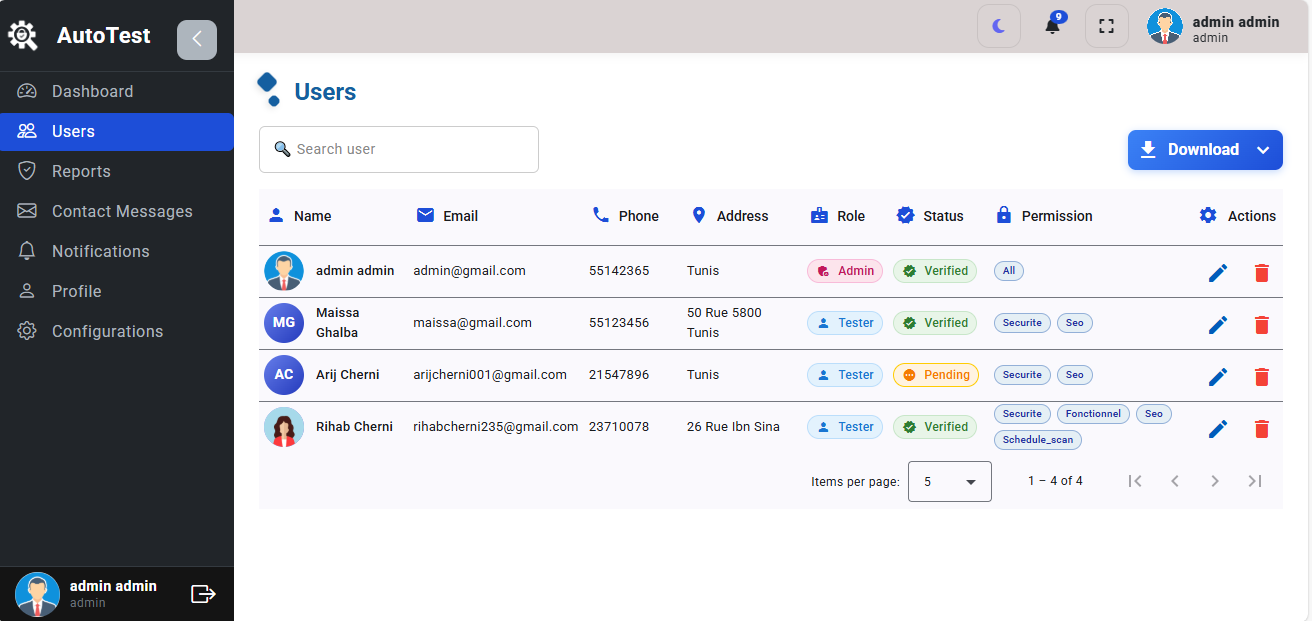
\includegraphics[width=\linewidth]{chapitres/ch3Sp1/section/sprint1/img/interface/user-liste.PNG}
            \caption{\centering Interface de gestion des utilisateurs et permissions (admin)}
            \label{fig:gestionUser}
        \end{figure}
        \vspace{-0.3cm}
       \item \textbf{Interfaces liées à la gestion des permissions et guards} :
Cette partie décrit les interfaces conditionnées par le système de gestion des permissions et les guards de sécurité implémentés dans l’application.
\begin{itemize}[label=$\diamond$, left=0.01cm]
    \item \textbf{Menu latéral dynamique selon les permissions} : La figure~\ref{fig:sidebar}\footnote{Voir annexe E : Figure~\ref{fig:sidebar}} illustre l’adaptation dynamique du menu latéral en fonction des droits d’accès de l’utilisateur. Trois cas sont représentés : (a) un utilisateur sans permissions, où seuls les éléments de base (profil, paramètres) sont visibles, (b) un utilisateur disposant de permissions spécifiques accédant uniquement aux modules autorisés, et (c) un utilisateur avec l’ensemble des droits, ayant un accès complet aux modules (SEO, sécurité, tests fonctionnels, génération de rapports, ...).
        \item \textbf{Interfaces de gestion des permissions}: La figure~\ref{fig:permission-interfaces}\footnote{Voir annexe E: Figures \ref{fig:permission-interfaces}} présente les interfaces illustrant les mécanismes de gestion et de demande de permissions.    
        \begin{itemize}[label=$*$, left=0.01cm]
            \item (a) Boîte de dialogue des permissions pour l’administrateur, avec toutes les permissions cochées et désactivées grâce à la permission spéciale \texttt{tous}, accordant un accès complet.
            \item (b) Boîte de dialogue d’édition des permissions, accessible uniquement à l’administrateur, permettant d’ajouter ou de révoquer dynamiquement les droits d’un utilisateur de rôle \texttt{testeur}.
            \item (c) Interface de demande de permissions, permettant au testeur de visualiser les accès manquants et de soumettre une requête à l’administrateur. Une notification est automatiquement envoyée. Ce composant a été conçu avec une logique évolutive en vue de la commercialisation de l’application : certaines permissions pourront, à l’avenir, être conditionnées par un abonnement payant. Une option de paiement ou un lien vers la facturation pourra alors s’activer dynamiquement lors de la sélection.
    \end{itemize}
\end{itemize}
\item \textbf{Soumettre un message de contact}:
        L’interface illustrée dans la figure~\ref{fig:contact}\footnote{Voir annexe E: Figures \ref{fig:contact}} permet à tout utilisateur (même non connecté) de soumettre un message à l’administrateur.
    \item \textbf{Interface de liste des messages (côté administrateur)}:
        La figure~\ref{fig:admin-contact-list}\footnote{Voir annexe E: Figures \ref{fig:admin-contact-list}} montre l’interface accessible uniquement à l’administrateur, lui permettant de consulter la liste des messages reçus via le formulaire de contact.
\end{itemize}
